\documentclass[../practica_02.tex]{subfiles}

\begin{document}

    \begin{enumerate}
        \item $r(t) = (\cos(t), \sin(t),1)$
            \begin{itemize}
                \item $ f(t) = \cos(t) \Rightarrow f: \real \rightarrow [-1,1] $
                \item $ g(t) = \sin(t) \Rightarrow f: \real \rightarrow [-1,1] $
                \item $ h(t) = \cos(t) \Rightarrow f: \real \rightarrow 1 $
            \end{itemize}

            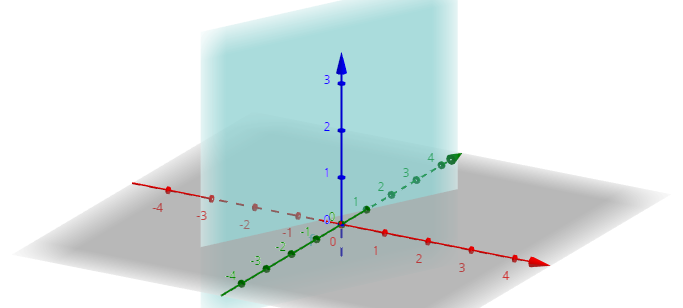
\includegraphics[scale=0.4]{ej10/resources/a.png} $ $

            $ $

        \item $r(t) = (t, t^2,t-t^2)$
            \begin{itemize}
                \item $ f(t) = t \Rightarrow f: \real \rightarrow [-1,1] $
                \item $ g(t) = t^2 \Rightarrow f: \real \rightarrow [0,\infty+] $
                \item $ h(t) = t-t^2 \Rightarrow f: \real \rightarrow [\infty-,\frac{1}{4}] $
            \end{itemize}

            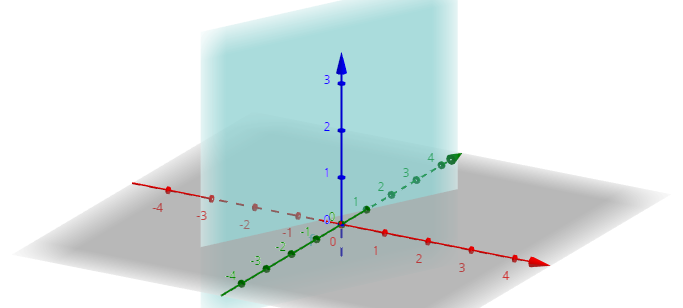
\includegraphics[scale=0.4]{ej10/resources/a.png} $ $

            $ $

        \item $r(t) = (t^2+t, t^2-t,(t^2-t)^2)$
            \begin{itemize}
                \item $ f(t) = t^2+t \Rightarrow f: \real \rightarrow [-\frac{1}{4},\infty+] $
                \item $ g(t) = t^2-t \Rightarrow f: \real \rightarrow [-\frac{1}{4},\infty+] $
                \item $ h(t) = (t^2-t)^2 \Rightarrow f: \real \rightarrow [0, \infty+] $
            \end{itemize}

            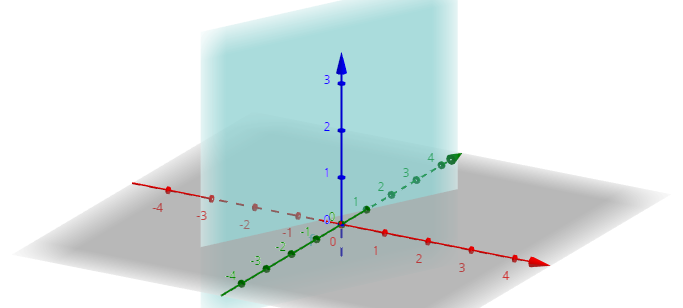
\includegraphics[scale=0.4]{ej10/resources/a.png} $ $

    \end{enumerate}

\end{document}